\documentclass[10pt,conference,compsocconf]{IEEEtran}

\usepackage{url}
\usepackage[table,xcdraw]{xcolor}
\usepackage{eurosym}
\usepackage{amsfonts}
\usepackage{balance}
\usepackage[pdftex]{graphicx}
   %declare the path(s) where your graphic files are
  % and their extensions so you won't have to specify these with
 % every instance of \includegraphics
\DeclareGraphicsExtensions{.pdf,.jpg,.png}

\hyphenation{second-ly ap-pen-dix}

\clubpenalty = 10000
\widowpenalty = 10000
\displaywidowpenalty = 10000

\newcommand{\todo}[1]{\textbf{#1}}

\begin{document}
%
% paper title
% can use linebreaks \\ within to get better formatting as desired
\title{End-User Refactoring}

\author{\IEEEauthorblockN{Felienne Hermans, David Hoepelman}
\IEEEauthorblockA{Delft University of Technology\\
Mekelweg 4\\
2628 CD Delft, the Netherlands\\
f.f.j.hermans@tudelft.nl}


\and
\IEEEauthorblockN{Katryn Stolee}
\IEEEauthorblockA{Iowa State University\\
209 Atanasoff Hall\\
Ames, IA 50011-1041\\
Email Katie}
}

\maketitle

\begin{abstract}
\end{abstract}


\begin{IEEEkeywords}
end-user computing; refactoring; 
\end{IEEEkeywords}

\section{Introduction}
The number of end-user programmers is said to greatly exceed the number of professional programmers. ``The proportion of American end user workers reporting they “do programming” has remained relatively constant, rising from around 10\% in 1989 to only around 15\% in 2001''~\cite{Scaf2005} This 15\% of 2001 totals to about 11 million end users, while the number of professional developers was estimated at 3 million for the same period~\cite{Scaf2005}.

These end-user programmers perform a wide variety of tasks within the organizations they work for, ranging from building or maintaining applications to simple data manipulation in a spreadsheet. While performing these tasks, end-users user programmers face many of the challenges of professional developers, such as identifying faults, debugging, or understanding code written by someone else~\cite{Ko2011}.

Contrary to what people might think, end-user artifacts are not always created ad-hoc, but may in fact have a long life-span. A recent case study showed that spreadsheets have an average lifespan of 5 years~\cite{Hermans2011}. In their lifespan, these artifacts are modified, often by different people. This makes them vulnerable for \emph{smells}, like programming artifacts. 

These smells in end-user programming have been a topic of research over the past few years. Most notable are smells in Yahoo Pipes~\cite{Stolee2011}, smells in spreadsheets \cite{Hermans2012inter}, and performance smells in Labview code \cite{chambers2013smell}. Experiments in all these areas have shown that end-users in fact understand smells and often prefer versions of their code that are non-smelly. Alleviating those smells can be achieved with refactoring, which leads us to the topic of this paper: how can we support do end-users in refactoring their artifacts? \todo{This is up for discussion.}

\section{Background}
\label{sec:background}

%Refactoring, improving the internal composition of a software program without altering its functionality or output \todo{quote a definition}, has been a part of software engineering since at least 1989 \cite{arnold1989software}, but was popularized by Fowler's 1999 "Refactoring: Improving the design of existing programs" \cite{fowler1999refactoring}. 
Since their introduction by Martin Fowler in 1999, extensive research has been done into code smells. Code smells, according to Fowler, indicate suspicious or weak parts that the developer might want to change in order to improve readability and minimize the chance of future errors. ~\cite{Fowl1999} `'A code smell is a surface indication that usually corresponds to a deeper problem in the system'', says Fowler. Like source code produced by professional developers, programs made by end-users can also contain smells.

\section{Smells in end-user artifacts}
\label{sec:smells}
Research into end-user programming smells can take on of two approaches.
The first approach take existing smells for object-oriented programming languages, usually those defined by Fowler, and transform them to be applicable to the end-user environment \cite{Hermans2012intra,Hermans2012inter}.

Another approach is to define smells directly for the end-user environment.
This can be done by interviewing experienced end-users to see which smells they perceive \cite{chambers2013smell}, by looking at user reports like forum or newsgroup posts \cite{Stolee2011} or by analyzing publicly available artifacts \cite{Stolee2011}.
A combination of both approaches is also possible.

This section provides an overview of different types of smells that can be applicable to end-user artifacts.

\subsection{Smells in spreadsheets}

In modern spreadsheet programs a \textit{cell} can contain a single \textit{formula} which performs a calculation, and a table of cells is bundled in a \textit{worksheet}.
A \textit{workbook} consist of a collection of worksheets.
Formulas can reference other cells in the same or in a different worksheet.
References to a different workbook are also possible but less common. \todo{True? source}
 
Hermans et al. \cite{Hermans2012inter} \cite{Hermans2012intra} analogize a workbook to a program and a worksheet to a class inside that program and a cell to a method.
Working from this analogy, the classic Fowler smells can be divided into class and method smells.
The class smells correspond to \textit{inter-sheet} smells and method smells correspond to \textit{intra-sheet} smells.

In \cite{Hermans2012inter} Hermans et al. define inter-worksheet smells and define and evaluate threshold for them based on the EUSIS spreadsheet corpus \cite{fisher2005euses}.
Fowler's class smells are translated into spreadsheets using the above analogy. 
For example the \textit{Feature Envy} smell indicates that a class uses members of another class more than it uses the members of its own class.
Similarly a cell can use cells of other worksheets more than it uses those of its own sheet, and thus that cell could better be placed in the other sheet.

In \cite{Hermans2012intra} Hermans et al. define intra-worksheet or formula smells and again define and evaluate thresholds for them based on the EUSIS corpus.
Supporting the validity of the above analogy several method-level smells translate well into cell-level smells.
\textit{Multiple References} is similar to the \textit{Many parameters} code smell. Like a method with many parameters can be hard to understand or change a cell that uses many references can have the same problem.
Hermans also defines a smell with no direct analogy, \textit{Long Calculation Chain}, which happens because references formulas can reference other formulas ad infinitum.
This can lead to difficult to understand calculation chains with many steps.
Although no formal smell definition is available, this is similar to the problems associated with programs with many layers, sometimes called \textit{Lasanga Code}.
\todo{This seems more of an inter-sheet/class smell. It's in the intra-smells paper though}

\subsection{Smells in LabVIEW programs}

LabVIEW is a proprietary hardware system design environment which features the visual programming language "G" as one of its primary features.
Some users claim they are two to three times as productive in G as they are in general-purpose alternatives like C or FORTRAN \cite{chambers2013smell}.
However, G programs do not always perform well, which has motivated Chambers and Scaffidi \cite{chambers2013smell} to define performance-degrading smells in G and implement heuristics to identify these smells.

The smells identified roughly fall into three categories. The first are smells specific to the environment, for example the \textit{"Sequence instead of State machine"} smell which is a smell because state machines can be much better optimized by the G compiler.

The second and third categories are more broadly applicable, with the second category being smells you could find a any program that uses concurrency.
One can easily see how \textit{"Non reentrant VI"}, a VI being a building block similar to a function, is a smell in a language that heavily relies on concurrency and parallelization since such a VI will require blocking and thus possibly slows down the program.

The third and largest category are (performance) smells that are applicable to general purpose languages.
\textit{"Multiple Nested Loops"} is a smell in almost any language that supports loops, and \textit{"Build Array inside Loop"} would be similar to allocating multiple small segments of memory with C's \texttt{malloc} inside a loop with potentially equally bad performance implications.

Chambers and Scaffidie implemented their smell-finding heuristics in a tool integrated into LabVIEW and evaluated it with 26 experienced LabVIEW programmers divided in two groups of 13 of which only one had access to their tool.

The results were promising, with all 13 tool-users being able to identify the problems in the given programs and 12 being able to fix the problem.
In contrast only 5 out of 13 non-tool-users were able to identify the problem and 3 out of 5 being able to fix the problem, although the latter is statistically insignificant.
Tool users also needed 34\% less time to identify the problem and 65\% less time to fix the problem, but these results were not statistically significant.
This evaluation shows that experienced end user programmers can benefit from tool support in identifying problems.


\subsection{Smells in Yahoo pipes}
In ~\cite{Stolee2011}, Stolee and Elbaum describe a number of smells. In addition to the smells, they present evidence that users of Yahoo pipes prefer non-smelly pipes over smelly ones, as shown in Figure \ref{fig:Table1-Stolee2011}.

\begin{figure}[ht!]
\centering
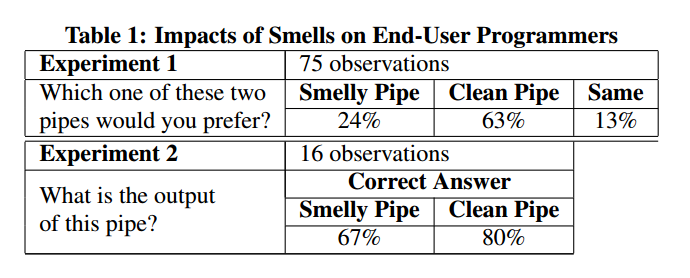
\includegraphics[width=\columnwidth]{Table1-Stolee2011.png}
\caption{End-users showing a preference for non-smelly pipes(from \cite{Stolee2011})}
\label{fig:Table1-Stolee2011}
\end{figure}

\todo{more summary here}

\section{Refactoring end-user programs}
\label{sec:refactoring}
Now that we have described various smells in different end-user artifacts, we direct our attention to the refactoring of them. 

\section{Empirical evidence}
\label{sec:empirical}


\section{Related Work}
\label{sec:related_work}

\section{Discussion}
\label{sec:discussion}


\section{Concluding Remarks}
\label{sec:conclusions}

\newpage
\balance
\bibliographystyle{plain}
\bibliography{literaturelist}

\end{document}


